\documentclass[10pt,a4paper]{article}

\usepackage[utf8]{inputenc}
\usepackage[T1]{fontenc}	
\usepackage[italian]{babel}
\usepackage{amsmath}
\usepackage{amsfonts}
\usepackage{amssymb}
\usepackage{graphicx}

\usepackage[left=2cm,right=2cm,top=2cm,bottom=2cm]{geometry}
\geometry{a4paper}

\usepackage{booktabs} % for much better looking tables
\usepackage{verbatim}
\usepackage{subfig} % make it possible to include more than one captioned figure/table in a single 

\usepackage{fancyhdr} % This should be set AFTER setting up the page geometry
\pagestyle{fancy} % options: empty , plain , fancy
\renewcommand{\headrulewidth}{0pt} % customise the layout...
\lhead{}\chead{}\rhead{}
\lfoot{}\cfoot{\thepage}\rfoot{}

%%% SECTION TITLE APPEARANCE
\usepackage{sectsty}
%\allsectionsfont{\sffamily\mdseries\upshape} % (See the fntguide.pdf for font help)
% (This matches ConTeXt defaults)
% pacchetti che mi fanno schifo ma uso lo stesso (Bob è scemo...)
\usepackage[cdot, thickqspace]{SIunits}
% macro che mi piacciono
\def\code#1{\texttt{#1}}


\title{Esercitazione 4: Amplificatore a transistor}

\author{Gruppo BE \\ Alessandro Candido, Roberto Ribatti}
\date{\today}
\begin{document}
\maketitle

\section{Scopo e strumentazione}

\section{Montaggio del circuito e punto di lavoro}

\section{Risposta a segnali sinusoidali a frequenza fissa}

\section{Risposta in frequenza}

Si è misurata la risposta in frequenza del circuito in esame in un range tra $\unit{10}{\hertz}$ ed $\unit{1}{\mega\hertz}$ con una tensione di ingresso costante di $\unit{1.00 \pm 0.03}{\volt}$. Di seguito si riportano i dati raccolti e il diagramma di Bode da questi ricavato.

\begin{figure}[h!]
	\centering
	\begin{minipage}[c]{0.3\textwidth}
		\centering
		\resizebox{\textwidth}{!}{
			\input{../tabelle/tab_f_domain.txt}}
		\captionof{table}{Dati raccolti}
	\end{minipage}
	\begin{minipage}[c]{0.69\textwidth}
		\centering
		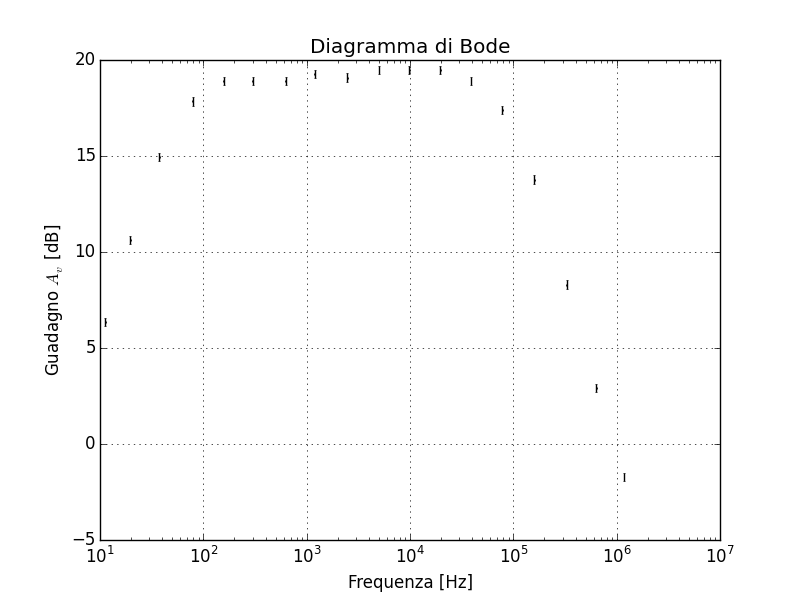
\includegraphics[width=1.1\textwidth]{../grafici/fast_plot_f_domain.pdf}
		\caption{Risposta in frequenza}
		\label{early}
	\end{minipage}
\end{figure}

Il grafico mostra un comportamento divisibile in tre bande di risposta:
\begin{itemize}
	\item basse frequenze ($\lesssim$ \unit{100}{\hertz}): il diagramma di Bode mostra un comportamento lineare, a queste frequenze le impedenze dei condensatori $C_{OUT}$ e $C_{IN}$ nel circuito non è trascurabile e diminuisce il guadagno del circuito.
	\item medie frequenze ($\unit{100}{\hertz} \lesssim f \lesssim \unit{100}{\kilo\hertz}$): in questo range di frequenze il guadagno del circuito è costante, tutte le approssimazioni che si fanno classicamente per la risoluzione del circuito sono valide e il comportamento è quello atteso;
	\item alte frequenze ($\gtrsim \unit{100}{\kilo\hertz}$): anche qui il diagramma di Bode mostra un comportamento lineare, la diminuzione del guadagno è dovuta alla capacità della giunzione.
\end{itemize}

Si è stimata la frequenza di taglio del circuito misurando la frequenza per la quale si ha un guadagno di $\unit{-3}{\deci\bel}$ e si è stimato l'errore valutando quando, al variare della frequenza, si misurava una variazione apprezzabile della tensione di uscita.
I risultati ottenuti sono stati: $f_1 = \unit{51 \pm 2}{\hertz}$ e $f_2= \unit{92 \pm 4}{\kilo\hertz}$.



\section{Aumento del guadagno}

Si è inserita la resistenza $Res = \unit{100.7 \pm 1.1}{\ohm}$ nel circuito in \figurename{\ref{stocazzo}} e si è proceduto alla misura del guadagno a frequenza costante di $\unit{5.03 \pm 0.05}{\kilo\hertz}$ al variare delle tensione di ingresso. I dati raccolti sono riportati di seguito.

\begin{figure}[h!]
	\centering
	%\resizebox{0.6\textwidth}{!}{
		\input{../tabelle/tab_C_E.txt}
	\caption{Dati raccolti}
\end{figure}

Il guadagno è stato valutato facendo una media dei guadagni misurati ed il risultato è stato $A_v = -79.2 \pm 1.4$, come è chiaro non è compatibile con il risultato della formula $A_v = -R_C/Res = 98.6 \pm 1.4$ perché questa formula è il risultato dell'approssimazione $h_{fe}*Z_c >> h_{ie}$, che non è valida in questo caso poichè $h_{fe} * Z_c \simeq h_{fe} * Res \simeq \unit{130 * 100}{\ohm} = \unit{13}{\kilo\ohm} $ che è confrontabile a $h_{ie}$ che secondo il datasheet vale $\sim \unit{4}{\kilo\ohm}$, applicando la formula non approssimata $A_v = -h_{fe}*R_C/(h_{fe}*Z_c + h_{ie}) \simeq 77$

\end{document}
